\documentclass[11pt,a4paper]{article}
\usepackage{graphicx}
\usepackage{amsmath}
\usepackage{geometry}
\geometry{margin=1in}
\graphicspath{{../}}

\title{Assignment 1: Laminar Flow through a Pipe}
\author{Sajeev}
\date{August 2025}

\begin{document}
\maketitle

\section{Governing Equations \& Setup}
The steady, incompressible, axisymmetric laminar flow is governed by the Continuity and Navier-Stokes equations:
\begin{align*}
\nabla \cdot \vec{U} &= 0 \\
\rho (\vec{U} \cdot \nabla) \vec{U} &= -\nabla P + \mu \nabla^2 \vec{U}
\end{align*}
Simulations were performed for $Re=100$. A uniform velocity inlet, pressure outlet, and no-slip wall boundaries were applied. Discretization was performed using the QUICK scheme for momentum and SIMPLE for pressure-velocity coupling, with convergence criteria of $10^{-6}$.

\section{Grid Independence \& Validation}
Three grids (Coarse, Medium, Fine) were evaluated. The velocity profile and pressure drop across the pipe length stabilized at the Medium grid (20 mm $\times$ 5 mm with 1.08 bias factor). The fully developed velocity profile perfectly matched the analytical Hagen-Poiseuille parabolic profile:
\[ u(r) = 2U_{\text{avg}} \left( 1 - \left(\frac{r}{R}\right)^2 \right) \]
For a mean velocity $U_{\text{avg}} = 0.5$ m/s, the analytical maximum velocity at the axis ($r=0$) is $u_{max} = 1.0$ m/s, which perfectly matched the CFD predictions. Furthermore, using $\Delta P / L = 8\mu U_{\text{avg}} / R^2$, with $\mu = 0.001$ kg/m-s and $R = 0.1$ m, the expected pressure drop of $0.4$ Pa/m was achieved in the fully developed region.

\begin{figure}[h!]
    \centering
    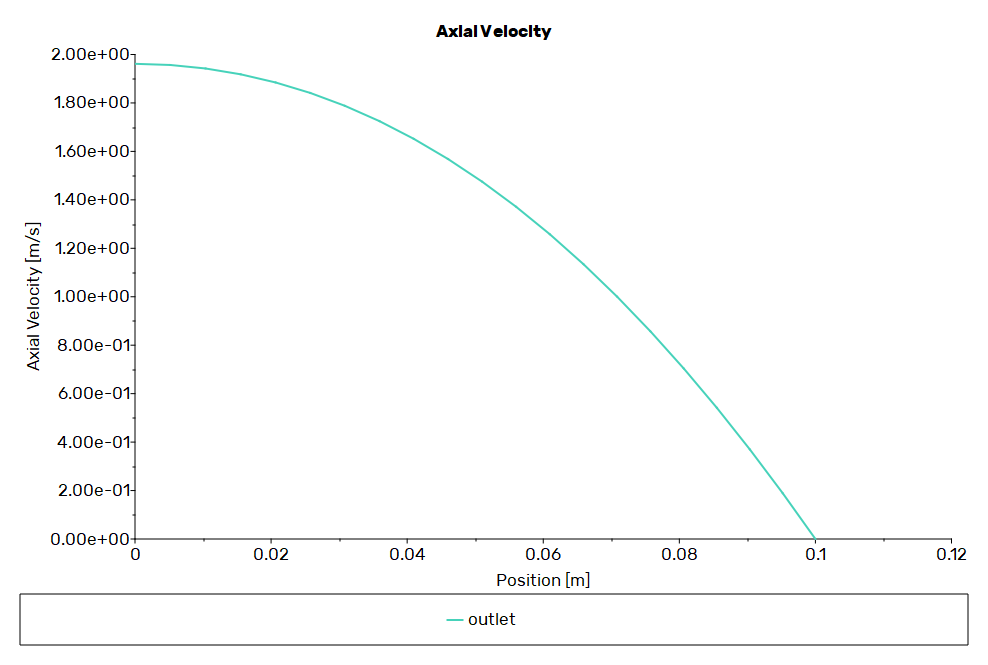
\includegraphics[width=0.45\linewidth]{vel-prof-graph.png}
    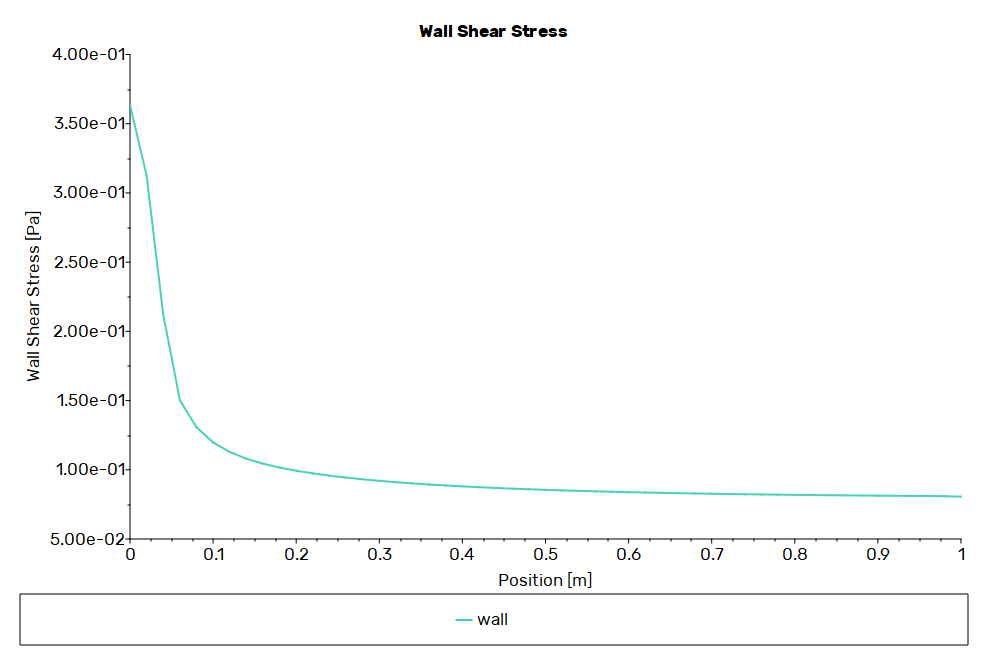
\includegraphics[width=0.45\linewidth]{wall-sheer-graph.png}
    \caption{Left: Fully developed velocity profile vs Analytical. Right: Wall shear stress evolution.}
\end{figure}

\section{Analysis of Results}
The velocity vectors and contours show the flow entering with a uniform velocity and a boundary layer growing from the wall, eventually converging at the axis to form a fully developed parabolic profile. The wall shear stress exhibits a very high value at the entrance due to sharp velocity gradients, decreasing exponentially and reaching a constant asymptote in the fully developed region. An alternative approach using periodic boundary conditions and mass flow specification can completely bypass this entry region simulation, yielding the fully developed profile instantly.

\end{document}
